\chapter{Análisis y Diseño del Sistema}\label{ch:Análisis y diseño del sistema}
En este capítulo se evaluaron los datos del marco teórico para seleccionar los componentes más adecuados para el proyecto. También se realizó un análisis detallado de los requerimientos y riesgos asociados al desarrollo del sistema, asegurando un diseño eficiente y viable para su implementación.

\section{Metodología de Desarrollo}
La metodología a usar	La metodología propuesta para el desarrollo del proyecto es Prototipos Evolutivos, en la cual se emplearán dos iteraciones mínimas. Esta metodología es adecuada para proyectos en los que la comprensión completa de los requisitos puede surgir gradualmente y en donde es importante recibir retroalimentación continua ~\cite{MetodologíasDeDesarrollo2015}. Al utilizar prototipos, se permite una aproximación más ágil al desarrollo, ya que se pueden generar soluciones tempranas que serán ajustadas en función de los comentarios de los usuarios y evaluaciones constantes.

\begin{figure}[H]
	\centering
	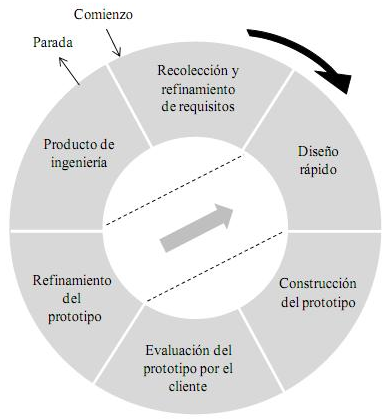
\includegraphics[width=0.5\textwidth]{img/chapter04/prototipo.png}
	\caption{Etapas de la metodología por prototipos \newline \centering \textit{Fuente: ~\cite{MetodologíasDeDesarrollo2015}}}
	\label{fig:prototpios-metodología}  % Etiqueta para la figura
\end{figure}

El uso de prototipos evolutivos permite abordar los requerimientos del sistema de manera iterativa. Cada prototipo no es desechado sino que se refina progresivamente hasta obtener una versión completa del sistema. Esto asegura que el producto final no solo cumpla con los requisitos establecidos inicialmente, sino también con las expectativas del cliente o usuario. \newline \newline
La retroalimentación temprana que se recibe desde las primeras etapas del proyecto es invaluable para identificar mejoras y posibles problemas antes de que se conviertan en obstáculos mayores. Esto permite un ahorro significativo de tiempo y recursos, ya que se pueden realizar correcciones antes de que los problemas se propaguen en el ciclo de desarrollo. \newline \newline
A continuación, se muestra una tabla comparativa de ventajas/desventajas de utilizar esta metodología.
\begin{longtable}{|m{6.5cm}|m{6.5cm}|}
	\hline
	\rowcolor{black!75} \color{white}\textbf{Ventajas} & \color{white}\textbf{Desventajas} \\
	\hline
	Permite obtener retroalimentación temprana y frecuente del cliente, lo que ayuda a ajustar los requerimientos de manera rápida. &
	Puede generar una dependencia excesiva de los prototipos, llevando a malentendidos sobre la funcionalidad final del producto. \\
	\hline
	Facilita la detección temprana de errores o problemas de diseño, lo que reduce costos de desarrollo en fases posteriores. &
	Requiere recursos adicionales (tiempo y esfuerzo) para desarrollar y revisar los prototipos. \\
	\hline
	Mejora la comprensión de los requisitos por parte del equipo de desarrollo y el cliente, reduciendo malentendidos. &
	Si no se maneja adecuadamente, puede desviar el proyecto del alcance original, añadiendo características no planificadas (creeping scope). \\
	\hline
	Aumenta la satisfacción del cliente al ver un producto tangible en las primeras fases del desarrollo. &
	El prototipo puede ser confundido con el producto final, lo que puede generar expectativas irreales respecto a tiempos y calidad. \\
	\hline
	Fomenta la iteración y mejora continua del producto, asegurando que se ajuste mejor a las necesidades reales del cliente. &
	El uso excesivo de prototipos puede ralentizar el desarrollo del producto final si las iteraciones no están bien gestionadas. \\
	
	\hline
	\rowcolor{white} \caption{Ventajas/Desventajas de la metodología de Prototipos Evolutivos} \label{tabla:Ventajas-Desventajas-Prototipos} \\
\end{longtable}

\subsection{¿Por qué prototipos para este trabajo?}
Está perrona

\section{Análisis de Requerimientos}
Los requerimientos funcionales y no funcionales descritos en este documento son fundamentales para el desarrollo y éxito de la aplicación web de cálculo y visualización de Series de Fourier. Estos requerimientos definen no solo las funcionalidades que la aplicación debe cumplir, sino también las expectativas de rendimiento, seguridad y usabilidad. A través de su análisis, se asegura que el sistema propuesto sea capaz de resolver la problemática planteada de manera eficaz, proporcionando a los usuarios una herramienta confiable y eficiente para el análisis de series matemáticas.
\subsection{Requerimientos Funcionales}
Los requerimientos funcionales de un sistema describen lo que el sistema debe hacer. Describen las interacciones entre el sistema y su ambiente, en forma independiente a su implementación. El ambiente incluye al usuario y cualquier otro sistema externo con el cual interactúa el sistema.

% Requerimiento 1
\begin{longtable}{|m{3.5cm}|m{9.5cm}|}
	\hline
	\rowcolor{black!75} \color{white}\textbf{Requerimiento} & \color{white}\textbf{Ingreso de Funciones Matemáticas} \\
	\hline
	
	\textbf{Identificador} & RF1 \\
	\hline
	\textbf{Prioridad de desarrollo} & Alta \\
	\hline
	\textbf{Entrada} & Funciones matemáticas ingresadas por el usuario usando MathQuill \\
	\hline
	\textbf{Salida} & Funciones ingresadas en formato compatible con Maxima \\
	\hline
	\textbf{Descripción} & El usuario debe poder ingresar funciones matemáticas definidas en un solo trozo o en múltiples trozos usando una notación matemática intuitiva. Debe soportar funciones trigonométricas, polinomios, exponenciales y cualquier otra función que Maxima pueda interpretar. \\
	\hline
	\textbf{Precondición} & El usuario debe estar en el área de ingreso de funciones. \\
	\hline
	\textbf{Postcondición} & Las funciones son ingresadas correctamente y listas para su procesamiento. \\
	\hline
	\rowcolor{white} \caption{Requerimiento funcional No. 1} \label{tabla:RF1} \\
\end{longtable}


% Requerimiento 2
\begin{longtable}{|m{3.5cm}|m{9.5cm}|}
	\hline
	\rowcolor{black!75} \color{white}\textbf{Requerimiento} & \color{white}\textbf{Selección de Parámetros} \\
	\hline
	\textbf{Identificador} & RF2 \\
	\hline
	\textbf{Prioridad de desarrollo} & Alta \\
	\hline
	\textbf{Entrada} & Parámetros seleccionados por el usuario (tipo de serie, período T) \\
	\hline
	\textbf{Salida} & Parámetros listos para el cálculo de coeficientes \\
	\hline
	\textbf{Descripción} & Los usuarios deben poder seleccionar entre las diferentes representaciones de Series de Fourier y especificar el período T de la función, ya sea de -T/2 a T/2 o de 0 a T. \\
	\hline
	\textbf{Precondición} & El usuario debe haber ingresado una función matemática y estar en el área de selección de parámetros. \\
	\hline
	\textbf{Postcondición} & Los parámetros seleccionados están listos para el cálculo de coeficientes. \\
	\hline
	\rowcolor{white} \caption{Requerimiento funcional No. 2} \label{tabla:RF2} \\
\end{longtable}


% Requerimiento 3
\begin{longtable}{|m{3.5cm}|m{9.5cm}|}
	\hline
	\rowcolor{black!75} \color{white}\textbf{Requerimiento} & \color{white}\textbf{Cálculo de Coeficientes} \\
	\hline
	\textbf{Identificador} & RF3 \\
	\hline
	\textbf{Prioridad de desarrollo} & Alta \\
	\hline
	\textbf{Entrada} & Función matemática y parámetros seleccionados por el usuario \\
	\hline
	\textbf{Salida} & Coeficientes de la serie de Fourier calculados \\
	\hline
	\textbf{Descripción} & La aplicación debe calcular automáticamente los coeficientes de la serie de Fourier según la función ingresada y los parámetros especificados, enviando la información a Maxima y recibiendo los resultados. \\
	\hline
	\textbf{Precondición} & El usuario debe haber ingresado una función y seleccionado los parámetros necesarios. \\
	\hline
	\textbf{Postcondición} & Los coeficientes de la serie de Fourier se calculan y se devuelven al sistema. \\
	\hline
	\rowcolor{white} \caption{Requerimiento funcional No. 3} \label{tabla:RF3} \\
\end{longtable}


% Requerimiento 4
\begin{longtable}{|m{3.5cm}|m{9.5cm}|}
	\hline
	\rowcolor{black!75} \color{white}\textbf{Requerimiento} & \color{white}\textbf{Interactividad en la Gráfica} \\
	\hline
	\textbf{Identificador} & RF4 \\
	\hline
	\textbf{Prioridad de desarrollo} & Media \\
	\hline
	\textbf{Entrada} & Control del usuario sobre la gráfica (acercar, alejar, cantidad de términos n) \\
	\hline
	\textbf{Salida} & Gráfica interactiva modificada según la selección del usuario \\
	\hline
	\textbf{Descripción} & El usuario debe poder acercar, alejar y desplazar la gráfica, así como seleccionar la cantidad de términos n de la suma parcial a visualizar. \\
	\hline
	\textbf{Precondición} & El usuario debe haber ingresado la función y los parámetros. \\
	\hline
	\textbf{Postcondición} & La gráfica es ajustada interactivamente según la entrada del usuario. \\
	\hline
	\rowcolor{white} \caption{Requerimiento funcional No. 4} \label{tabla:RF4} \\
\end{longtable}

% Requerimiento 5
\begin{longtable}{|m{3.5cm}|m{9.5cm}|}
	\hline
	\rowcolor{black!75} \color{white}\textbf{Requerimiento} & \color{white}\textbf{Visualización de las Gráficas} \\
	\hline
	\textbf{Identificador} & RF5 \\
	\hline
	\textbf{Prioridad de desarrollo} & Alta \\
	\hline
	\textbf{Entrada} & Función original y términos de la Serie de Fourier \\
	\hline
	\textbf{Salida} & Gráficas de la función original y las sumas parciales de la Serie de Fourier \\
	\hline
	\textbf{Descripción} & El usuario debe poder visualizar la gráfica de la función original y las sumas parciales de la Serie de Fourier en un lienzo canvas, que se actualizará en tiempo real a medida que se agregan o quitan términos. \\
	\hline
	\textbf{Precondición} & El usuario debe haber ingresado la función y los parámetros necesarios. \\
	\hline
	\textbf{Postcondición} & La gráfica se actualiza en tiempo real según los términos seleccionados. \\
	\hline
	\rowcolor{white} \caption{Requerimiento funcional No. 5} \label{tabla:RF5} \\
\end{longtable}


% Requerimiento 6
\begin{longtable}{|m{3.5cm}|m{9.5cm}|}
	\hline
	\rowcolor{black!75} \color{white}\textbf{Requerimiento} & \color{white}\textbf{Visualización de resultados} \\
	\hline
	\textbf{Identificador} & RF6 \\
	\hline
	\textbf{Prioridad de desarrollo} & Alta \\
	\hline
	\textbf{Entrada} & Función matemática y parámetros seleccionados \\
	\hline
	\textbf{Salida} & Expresión matemática de la serie de Fourier y coeficientes individuales \\
	\hline
	\textbf{Descripción} & La aplicación debe mostrar la serie de Fourier y los valores individuales de los coeficientes en notación matemática, utilizando MathQuill. \\
	\hline
	\textbf{Precondición} & El usuario debe haber ingresado la función y los parámetros necesarios. \\
	\hline
	\textbf{Postcondición} & Se muestran la serie de Fourier y los coeficientes en notación matemática. \\
	\hline
	\rowcolor{white} \caption{Requerimiento funcional No. 6} \label{tabla:RF6} \\
\end{longtable}


% Requerimiento 7
\begin{longtable}{|m{3.5cm}|m{9.5cm}|}
	\hline
	\rowcolor{black!75} \color{white}\textbf{Requerimiento} & \color{white}\textbf{Manejo de Errores} \\
	\hline
	\textbf{Identificador} & RF7 \\
	\hline
	\textbf{Prioridad de desarrollo} & Media \\
	\hline
	\textbf{Entrada} & Función ingresada por el usuario, parámetros seleccionados \\
	\hline
	\textbf{Salida} & Mensajes de error claros en caso de problemas con la función o los parámetros \\
	\hline
	\textbf{Descripción} & La aplicación debe detectar errores en la entrada de funciones o parámetros no válidos y mostrar mensajes de error claros. También debe notificar si las integrales no convergen o si Maxima no puede procesar la función. \\
	\hline
	\textbf{Precondición} & El usuario ha ingresado una función o parámetros y ha intentado procesar los datos. \\
	\hline
	\textbf{Postcondición} & Se muestra un mensaje de error claro si ocurre algún problema. \\
	\hline
	\rowcolor{white} \caption{Requerimiento funcional No. 7} \label{tabla:RF7} \\
\end{longtable}


% Requerimiento 8
\begin{longtable}{|m{3.5cm}|m{9.5cm}|}
	\hline
	\rowcolor{black!75} \color{white}\textbf{Requerimiento} & \color{white}\textbf{Optimización de Resultados} \\
	\hline
	\textbf{Identificador} & RF8 \\
	\hline
	\textbf{Prioridad de desarrollo} & Baja \\
	\hline
	\textbf{Entrada} & Parámetros y resultados de coeficientes previos \\
	\hline
	\textbf{Salida} & Optimización de cálculo y presentación de resultados mejorada \\
	\hline
	\textbf{Descripción} & La aplicación debe optimizar el cálculo de los coeficientes para mejorar el rendimiento y la experiencia del usuario, manejando grandes cantidades de términos de manera eficiente. \\
	\hline
	\textbf{Precondición} & El usuario ha ingresado parámetros complejos o grandes cantidades de términos. \\
	\hline
	\textbf{Postcondición} & Los resultados optimizados se calculan y presentan rápidamente. \\
	\hline
	\rowcolor{white} \caption{Requerimiento funcional No. 8} \label{tabla:RF8} \\
\end{longtable}


\subsection{Requerimientos No Funcionales}
Los requerimientos no funcionales describen una restricción sobre el sistema que limita nuestras elecciones en la construcción de una solución al problema. Describen atributos sólo del sistema o del ambiente del sistema que no están relacionados directamente con los requisitos funcionales. Los requisitos no funcionales incluyen restricciones cuantitativas, tipo de plataforma.

%Tabla de no funcionales
\begin{longtable}{|m{5cm}|m{10cm}|}
	\hline
	\rowcolor{black!75} \color{white}\textbf{Nombre} & \color{white}\textbf{Descripción} \\
	\hline
%	\rowcolor{black!75}
%	\head {Nombre} & \head {Descripción} \\ \hline
%	\endfirsthead
%	\multicolumn{2}{c}{{\tablename\ \thetable{} -- continuación}} \\
%	\rowcolor{black!75}
%	\head {Nombre} & \head {Descripción}\\ \hline
%	\endhead
%	\hline \multicolumn{2}{r}{{Continúa en la siguiente página}} \\
%	\endfoot
%	\hline
%	\endlastfoot
	\textbf{Rendimiento y Escalabilidad} & El sistema debe calcular los coeficientes de Fourier en un tiempo razonable, incluso para funciones con múltiples trozos o con un alto número de términos en la serie. La visualización gráfica debe ser fluida y responsiva, incluso al agregar o quitar muchos términos de la serie. Las interacciones en el lienzo canvas deben realizarse sin latencia perceptible. \\
	\hline
	\textbf{Interfaz de Usuario Amigable e Intuitiva} & La interfaz debe ser intuitiva y fácil de usar, con botones y controles claramente identificados. Los mensajes de error y advertencia deben ser comprensibles, evitando el uso de jerga técnica complicada. La notación matemática debe ser clara y precisa, usando MathQuill para entradas y visualización de resultados. \\
	\hline
	\textbf{Manejo de la Concurrencia} & La aplicación debe soportar múltiples usuarios concurrentes enviando cálculos al backend sin generar bloqueos ni conflictos en las llamadas a Maxima. \\
	\hline
	\textbf{Portabilidad y Compatibilidad} & La aplicación debe ser compatible con los principales navegadores modernos (Chrome, Firefox, Edge). Aunque no es recomendable usar la aplicación en dispositivos móviles, el diseño debe ser responsivo para ajustarse a diferentes tamaños de pantalla, incluidos dispositivos móviles y tabletas. \\
	\hline
	\textbf{Modularidad y Extensibilidad del Código} & El frontend debe estar diseñado para facilitar la migración a frameworks como Angular en el futuro. El código debe ser modular y seguir buenas prácticas de desarrollo para facilitar la adición de nuevas características. Aunque el sistema no requiere una base de datos en su versión actual, el backend debe ser fácilmente extensible para permitir el almacenamiento de sesiones o configuraciones del usuario en el futuro. \\
	\hline
	\textbf{Seguridad de la Aplicación} & Las peticiones a la API deben estar protegidas contra inyecciones de código. Implementar seguridad básica en el backend para evitar solicitudes maliciosas o repetitivas que puedan afectar el rendimiento del servicio. \\
	\hline
	\textbf{Mantenibilidad de Código} & La aplicación debe tener una guía de usuario clara para explicar cómo ingresar funciones, seleccionar series y usar la interfaz. El código debe estar bien documentado para que futuros desarrolladores puedan entender la lógica y estructura de la aplicación fácilmente. \\
	\hline
%	\textbf{Tiempo de Respuesta del Sistema} & El tiempo de respuesta del servidor para calcular coeficientes de Fourier no debe exceder los 5 segundos en condiciones normales. La gráfica debe actualizarse en menos de 500 ms para proporcionar una experiencia interactiva y sin latencia. \\
%	\hline
%	\textbf{Consumo de Recursos} & La aplicación debe ser eficiente en el uso de memoria y CPU, especialmente al realizar cálculos de series grandes. El uso de canvas debe estar optimizado para no causar retrasos en la interfaz. \\
%	\hline
%	\textbf{Compatibilidad con Carga Asíncrona} & La comunicación entre el frontend y el backend debe ser asíncrona para no bloquear la interfaz de usuario. Las llamadas a Maxima deben ser gestionadas de manera eficiente para evitar cuellos de botella. \\
%	\hline
	\rowcolor{white} \caption{Tabla de requerimientos no funcionales} \label{tabla:RNF} \\
\end{longtable}




\section{Análisis de Riesgos}
\subsection{Identificación de Riesgos}
\subsection{Jerarquización de Riesgos}

\section{Estimación de Costos}
\subsection{Método de Estimación de Costos}
\subsection{Detalle de los Costos Estimados}

\section{Diseño del Sistema}
\subsection{Arquitectura General del Sistema}
\subsubsection{Arquitectura Cliente-Servidor}
\subsubsection{Flujo de Datos}

\subsection{Diseño de la Interfaz de Usuario}
\subsubsection{Estructura de la Interfaz}
\subsubsection{Prototipo de la Interfaz}
